\section{\large Low bitrate telephone transmission}
%For each problem, outline the problem in your own words, your approach, what you did and why you did it.
A speech signal, \texttt{spoken\_ sentence\_ 44100.wav}, was to be downsampled to around 8 kHz (more precisely 44.1/7 kHz = 6.3 kHz) by choosing every seventh sample, and then upsampled to 44.1 kHz again by repeating each sample seven times. In order to avoid the undesirable effect of aliasing, a low-pass filter must be applied before downsampling to remove/reduce the amplitude of frequencies above the Nyquist limit of 3.15 kHz. This lessens the presence of overlapping frequencies when the sampling frequency is lowered. Therefore a B-spline low-pass filter was created and applied to the signal. The MATLAB code employed to generate B-spline transfer functions of length \texttt{L} and order \texttt{n} is shown in Figure~\ref{fig:B-splineCode}.\\

\begin{figure}[H]
\center
\begin{lstlisting}
function [B] = Bspline(L, n); 
%INPUT: Length (L), order (n). OUTPUT: B-spline (B).
h = ones(L,1); %create ones
B = h;
if n ~= 0 
   for k = 1:n    %convolve recursively n times
       B = conv(B,h);
   end
end
B = B/norm(B,1); %normalize
end %eof
\end{lstlisting}
\caption{The \texttt{Bspline} function.}
\label{fig:B-splineCode}
\end{figure}

%STILL MISSING A PLOT OF THE BSPLINES
B-splines of length 6 and order 0 to 5 were generated and the time and frequency responses plotted in both linear and double logarithmic scale as shown in Figure~\ref{fig:B-splinePlot}. For the B-spline of length 6 order 3 zero-points can be observed on the double logarithmic plot located at frequencies approximately 7.35 kHz, 14.7 kHz and 22 kHz. The transfer function of this B-spline was used to filter \texttt{spoken\_ sentence\_ 44100.wav} by convolution using \texttt{conv} in the time-domain. The original and filtered signals are shown in Figure~\ref{fig:FilteredSpokenSentence}.\\

\begin{figure}[H]
\center
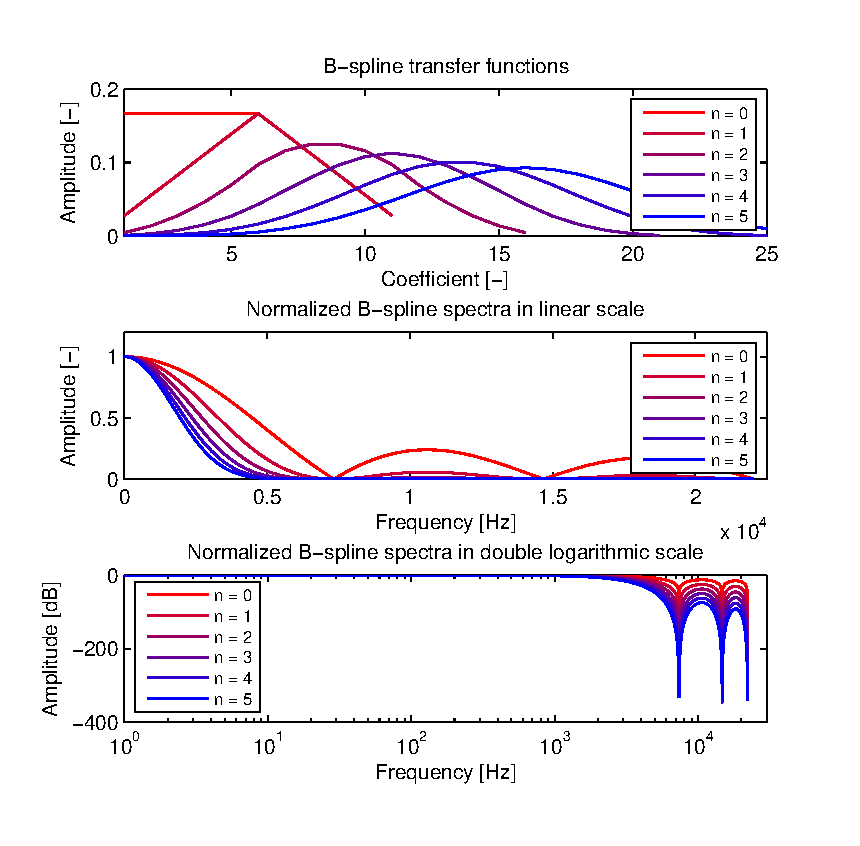
\includegraphics[scale=1]{report1-2-1-alt.eps}%
\caption{B-spline transfer functions of length 6 and order 0 to 5 and their normalized frequency response in linear and double logarithmic scale. The B-splines used to generate the spectra were zero-padded to a period of 1s in order to get acceptable resolution in the frequency domain.}
\label{fig:B-splinePlot}
\end{figure}

%What is the attenuation of that filter at 2, 4 and 5 kHz ?
The attenuation of the length 6 order 3 filter at 2 kHz, 4 kHz and 5 kHz can be read off the double logarithmic plot as approximately -4.25 dB, -18.50 dB and -31.50 dB respectively. In addition, the attenuation at 3.15 kHz and beyond exceeds -10 dB and this is sufficient for practical purposes. The zero-points are very apparent upon filtering as can be seen in Figure~\ref{fig:FilteredSpokenSentence}.\\

\begin{figure}[H]
\center
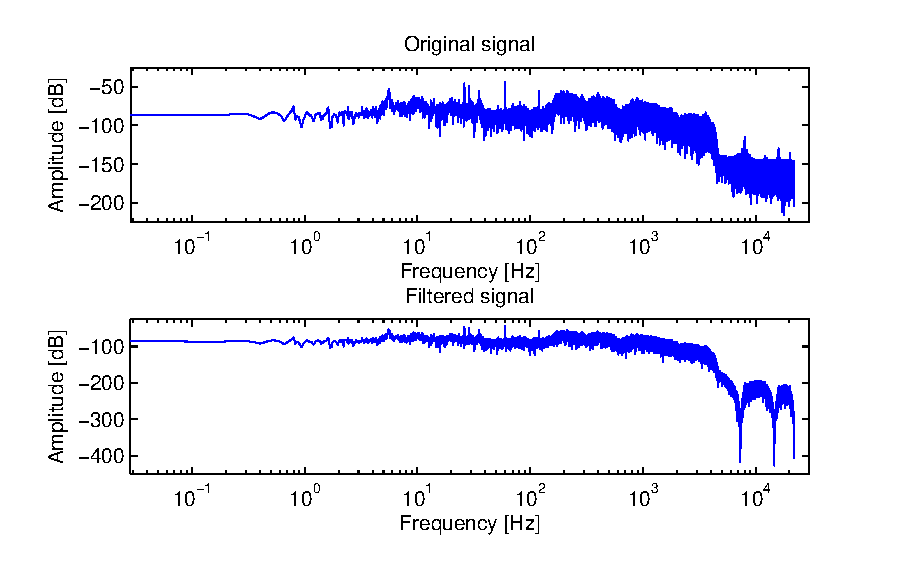
\includegraphics[scale=1]{report1-2-2.eps}\\
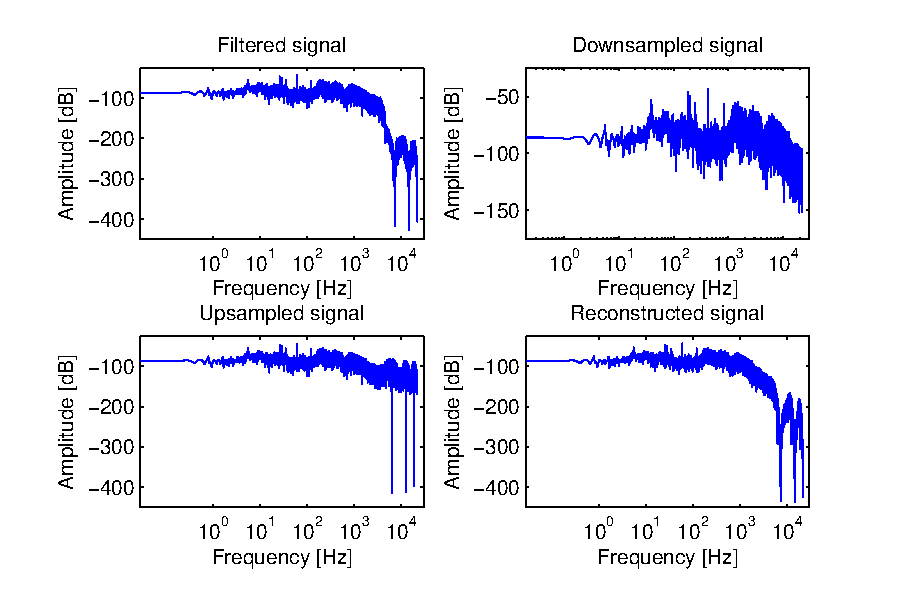
\includegraphics[scale=1]{report1-2-3.eps}
\caption{Original signal vs. Filtered signal (using B-spline of length 6 order 3) and the results of downsampling, upsampling and reconstruction by convolving with B-Spline transfer function of length 6 and order 5.}
\label{fig:FilteredSpokenSentence}
\end{figure}

%Are there artifacts in the spectrum coming from the crude upsampling?
Downsampling by removing every seventh sample (in MATLAB using the \texttt{downsample} function) results in the waveform shown in Figure~\ref{fig:FilteredSpokenSentence}. Frequencies slightly above the Nyquist limit are distorted and amplified. This is as expected since the B-spline filter imperfectly reduces frequencies above 3.15 kHz. Therefore upsampling to 44.1 kHz results in artifacts in the higher frequencies of the spectrum, but very little to no change in the lower frequencies as seen in Figure~\ref{fig:FilteredSpokenSentence}. \\

%Justify your choice of B-spline in terms of order an length. This filter is called the reconstruction filter.
A B-spline transfer function of length 6 and order 5 was selected to reconstruct the signal. The choice was made based on a qualitative assessment of the sound of the reconstructed signal. The shape and amplitude of the signal spectrum is also closer to the filtered signal before resampling when compared to the effect of B-spline filters of other lengths and orders (except possibly length 6 order 3).
